\documentclass[runningheads]{llncs}

\usepackage[T1]{fontenc}
\usepackage[utf8]{inputenc}
\usepackage[english]{babel}
\usepackage{amsmath,amssymb}
\usepackage{graphicx}
\usepackage{booktabs}
\usepackage{hyperref}
\usepackage{makecell}
\usepackage{float}
\graphicspath{{docs/figures/}}

\hypersetup{hidelinks}

\begin{document}

\title{Routed Kolmogorov--Arnold Fuzzy Networks for Stable Interpretable Classification\thanks{The research was carried out within the state assignment of Ministry of Science and Higher Education of the Russian Federation (theme No. 124112200072-2).}}
\titlerunning{Routed KA Fuzzy Networks}

\author{
    A. N. Averkin\inst{1}\orcidID{0000-0003-1571-3583} \and
    Yu. V. Trofimov\inst{2,3}\orcidID{0009-0005-6943-7432} \and
    A. D. Lebedev\inst{2}\orcidID{0009-0001-1046-5982} \and
    M. D. Lebedev\inst{4}\orcidID{0009-0005-1459-9119} \and
    A. S. Ilin\inst{5}\orcidID{0009-0007-9599-4958} \and
    A. V. Nechaevskiy\inst{2,3}\orcidID{0000-0001-6751-8195}
}

\authorrunning{A. N. Averkin et al.}

\institute{
    Federal Research Center ``Computer Science and Control'' of the Russian Academy of Sciences, Moscow, Russia
    \and Dubna State University, Dubna, Moscow Region, Russia
    \and Joint Institute for Nuclear Research, Dubna, Moscow Region, Russia\\
    \email{ura\_trofim@bk.ru, nechav@uni-dubna.ru}
    \and National University of Science and Technology MISIS, Moscow, Russian Federation
    \and Innopolis University, Innopolis, Russian Federation
}

\maketitle

\begin{abstract}
This paper studies how to increase the predictive capacity of neuro-fuzzy models without losing a reproducible rule-based explanation structure. We first implement a unified fuzzy-network framework with shallow, stacked, hierarchical, and Deep Fuzzy Feature Learning (DFFL) variants. Building on the limitations observed in these reference architectures, we introduce the main model of the paper: Teacher-Guided Routed Kolmogorov--Arnold Fuzzy Network (Routed KAFN).

Routed KAFN replaces a combinatorial multidimensional rule base with a deep additive fuzzy superposition. The first stage constructs concept variables as sums of one-dimensional fuzzy predicates selected by teacher-guided routing; the second stage applies another fuzzy superposition over these concepts. Binary and one-hot variables use only absent/present terms, while continuous variables use low/medium/high terms. A fixed projection-pursuit extension adds a small number of transparent sparse channels while preserving a stable rule topology.

On the \textit{covtype\_binary\_20000} benchmark, the best routed KA configuration reaches F1 $=0.8174\pm0.0101$ with 936 active rules and active-rule Jaccard $=0.9167$. It is close to the strongest stacked fuzzy baseline (F1 $=0.8222\pm0.0074$) and stronger than the histogram-gradient-boosting baseline used in the same focused block, while providing a much more reproducible rule structure than the stacked fuzzy model. The results support a quality--complexity--stability view of deep neuro-fuzzy design: the proposed KAFN is not a universal accuracy winner, but it gives a strong operating point where predictive quality and stable interpretability are jointly optimized.
\keywords{Kolmogorov--Arnold networks \and neuro-fuzzy systems \and interpretable machine learning \and fuzzy rules \and structural stability}
\end{abstract}

\section{Introduction}

Deep models achieve strong predictive results on tasks with complex nonlinear structure, but their internal logic often remains difficult to inspect~\cite{lecun2015deep}. In applied settings this limitation becomes a practical constraint. When a model is used for engineering analysis, monitoring, or decision support, experts need to follow the reasoning path that leads to the prediction, not only observe the prediction itself~\cite{rudin2019stop}. For this reason, interpretability is treated here as a structural property of the model.

Neuro-fuzzy methods address this requirement by combining data-driven learning with explicit rules and membership functions~\cite{jang1993anfis,mitra2000neurofuzzy}. ANFIS remains a key reference model in this line of work because it joins adaptive training with a readable fuzzy inference structure~\cite{jang1993anfis}. At the same time, classical ANFIS is shallow by design. As input dimensionality and interaction complexity increase, the rule base grows quickly and becomes harder to preserve in a coherent form~\cite{mitra2000neurofuzzy,magdalena2019semantic}.

This limitation motivates the main question of the study. Architectural complexity has to be increased without losing the traceability of internal representations. A stacked composition of fuzzy blocks can improve predictive quality, but its hidden states may become technical latent transformations rather than interpretable concepts. Hierarchical constructions can constrain rule growth by decomposing the input space, yet a compact hierarchy does not automatically make intermediate states semantically clear. Therefore, deeper neuro-fuzzy models should be assessed by the way they reorganize internal inference structure, not by expressive capacity alone.

For this reason, RMSE and F1 do not fully describe the behavior of such models. It is also necessary to evaluate whether internal representations remain inspectable, whether they are stable across independent runs, and what structural cost is required to maintain them~\cite{rudin2019stop,zeng2019deep,feng2020highly,alvarez2018self,koh2020concept,chen2019looks,chen2020concept}. This viewpoint is especially important for repeated expert review, rule auditing, and decision-support workflows. If predictive quality remains similar but the active rule structure changes strongly from run to run, the analytical reliability of the model decreases.

The contribution of this study is a unified fuzzy-block framework for analyzing depth in structurally interpretable neuro-fuzzy models and a new routed Kolmogorov--Arnold fuzzy architecture derived from this analysis. Within the framework, we design, mathematically formalize, and implement four reference architectures: shallow, stacked, hierarchical, and DFFL. The shallow, stacked, and hierarchical variants serve as controlled architectural configurations based on established organization principles, while DFFL represents a concept-oriented deep fuzzy design with staged concept-level re-estimation.

The main proposed model, Routed KAFN, uses the Kolmogorov--Arnold superposition principle as an architectural guide: multidimensional rules are replaced by sums of one-dimensional fuzzy predicates and a second fuzzy superposition over learned concept variables~\cite{kolmogorov1957superposition,arnold1957functions}. Teacher-guided routing fixes which predicates enter each concept, binary-aware terms remove redundant medium states for one-hot variables, and fixed sparse projection channels add limited interaction capacity without returning to a full combinatorial rule base.

All architectures are evaluated under matched preprocessing and optimization settings. This makes the comparison architectural rather than a set of fragmented model-specific experiments. The evaluation protocol combines predictive quality, rule-base complexity, and reproducibility of internal rule activation, and it is complemented by a case-level internal trace. The central result is a controlled quality--complexity--stability comparison that identifies Routed KAFN as the strongest stability-oriented fuzzy model in the focused Covtype setting.

\section{Related Work}

Research on interpretable neuro-fuzzy modeling is rooted in classical neuro-fuzzy systems, especially ANFIS. In this family of models, adaptive learning is connected with explicit fuzzy inference, and the learned parameters remain tied to readable rules and membership functions~\cite{jang1993anfis}. This property made neuro-fuzzy systems attractive for tasks where a prediction has to be accompanied by an inspectable reasoning structure. At the same time, early surveys showed a central limitation of this line of work: as the dimensionality and interaction complexity of a task increase, the rule base becomes harder to keep transparent and compact~\cite{mitra2000neurofuzzy}.

Hierarchical fuzzy systems address this limitation from the side of structural control. Instead of constructing one rule base over all input variables, they split the input space into smaller groups and combine local fuzzy outputs at higher levels~\cite{magdalena2019semantic,razak2022hierarchical}. This reduces combinatorial rule growth and makes the architecture easier to inspect. However, hierarchy mainly controls the size and organization of rules. It does not by itself define what the intermediate states mean, nor does it guarantee that these states remain stable across independent training runs.

A related direction introduces depth into rule-based models while preserving interpretability constraints. In these architectures, multilayer processing is combined with low-order rules, so the model can increase expressive capacity without fully losing readability~\cite{zeng2019deep,feng2020highly}. These works show that depth and rule-based inference can be combined in one architecture. They also reveal an important difficulty for the present study: hidden layers do not automatically become interpretable simply because the model is built from rule-based components~\cite{feng2020highly}.

Outside the neuro-fuzzy line, architecturally interpretable deep learning has developed another way of addressing the same problem. Self-explaining neural networks treat interpretability as an internal property of the predictor~\cite{alvarez2018self}. Concept bottleneck models force prediction to pass through explicit human-readable concepts~\cite{koh2020concept}. Prototype-based networks and concept-oriented representation learning follow a similar idea by aligning hidden representations with representative examples or predefined semantic directions~\cite{chen2019looks,chen2020concept}.

These studies mark a shift from explaining a finished black-box model toward designing models whose internal structure supports interpretation during inference. This distinction is essential here. Post hoc methods such as LIME and SHAP can explain individual predictions of a trained model, but they do not require the predictor itself to contain stable or semantically organized internal representations~\cite{ribeiro2016lime,lundberg2017shap,rudin2019stop}.

The Kolmogorov--Arnold superposition theorem gives another useful architectural viewpoint: a multivariate continuous function can be represented through sums and superpositions of univariate functions~\cite{kolmogorov1957superposition,arnold1957functions}. Recent Kolmogorov--Arnold Networks (KANs) use this principle to replace fixed node activations with learnable edge functions~\cite{liu2024kan}. In this paper we do not reproduce a spline-based KAN. Instead, we build a fuzzy counterpart: routed sums of one-dimensional membership predicates are combined into concept functions and then into a final fuzzy decision layer.

The remaining gap lies between these research lines. Neuro-fuzzy models preserve explicit rule-based reasoning, but they face structural growth when depth and high-dimensional inputs are introduced. Architecturally interpretable deep models provide concepts, prototypes, or self-explaining components, but fuzzy inference is not their core reasoning mechanism~\cite{zeng2019deep,alvarez2018self,koh2020concept,chen2019looks,chen2020concept}. This gap motivates the controlled comparison presented in this paper: fuzzy-block architectures are built on a shared fuzzy inference mechanism and compared as different ways of increasing depth while preserving structural interpretability, with Routed KAFN developed as the final stability-oriented architecture.

\section{Methodology}

All architectures considered in this study are built on a common neuro-fuzzy inference mechanism. They differ not in the basic form of the rule itself, but in the way fuzzy blocks are organized, how depth is introduced, and what role intermediate representations play in the final decision. Let $x \in \mathbb{R}^d$ denote the input vector and let $\hat{y}$ denote the model output. In the deep setting, the transformation is represented as a sequence of internal states,
\[
x \rightarrow c^{(1)} \rightarrow c^{(2)} \rightarrow \dots \rightarrow c^{(L)} \rightarrow \hat{y}.
\]
In this study, depth is treated as an architectural organization of intermediate representations rather than as a purely technical increase in the number of layers.

Figure~\ref{fig:architectures_overview} summarizes the four model families considered in the paper: a shallow model, a stacked model, a hierarchical model, and DFFL. Although these architectures share a common inference principle, they differ substantially in the way internal states are formed and propagated.

\begin{figure}[H]
    \centering
    \IfFileExists{1.jpg}
        {\includegraphics[width=\textwidth]{1.jpg}}
        {
\includegraphics[width=\textwidth]{fig1_architectures.png}}
    \caption{Overview of the four model families considered in the study: shallow, stacked, hierarchical, and DFFL.}
    \label{fig:architectures_overview}
\end{figure}

For a rule $r$ in a fuzzy block, the activation weight is defined as
\[
w_r = \sigma(g_r)\prod_{(i,j)\in A_r}\mu_{ij}(z_i),
\]
where $A_r$ denotes the antecedent structure of the rule, $\mu_{ij}(z_i)$ is the membership degree of the corresponding variable, and $\sigma(g_r)$ is a learnable rule gate. The gate is sample-independent and controls the global availability of rule $r$, while the product term is sample-dependent and encodes instance-specific antecedent matching. The activations are normalized as
\[
\bar{w}_r = \frac{w_r}{\sum_q w_q + \varepsilon},
\]
which keeps rule contributions comparable and numerically stable during training.

The same normalized activations are used to form either hidden concept representations or the final output. In hidden layers, the concept representation may be written as
\[
c = \sum_r \bar{w}_r v_r,
\]
where $z\in \mathbb{R}^{m}$ is the block input, $c\in\mathbb{R}^{k}$ is the block output, and $v_r\in\mathbb{R}^{k}$ is the concept vector associated with rule $r$. In a more expressive variant, the hidden consequent is parameterized as
\[
c = \sum_r \bar{w}_r \sigma(zW_r + b_r).
\]
Here $W_r\in\mathbb{R}^{m\times k}$ and $b_r\in\mathbb{R}^{k}$.
At the final stage, prediction is produced by a first-order Sugeno mapping,
\[
\hat{y} = \sum_r \bar{w}_r \left(a_{r0} + a_r^\top z\right),
\]
where $z$ denotes the representation at the last hidden level.

The shallow model serves as the reference configuration. It uses a single fuzzy block over the full input space and a single decision layer. Its main advantage is local readability, since the rule base remains relatively easy to inspect. Its limitation is restricted representational depth.

In the stacked model, depth is introduced through a sequential composition of fuzzy blocks. The output of one block becomes the input to the next. This design refines the representation step by step and often improves predictive performance, but the resulting intermediate states may become technical latent transformations rather than semantically stable concepts.

In the hierarchical model, depth is introduced through decomposition rather than simple sequential stacking. Local groups of features are processed by separate fuzzy blocks, and their outputs are then aggregated at a higher level. This reduces the pressure on a single global rule base and provides a more controlled compromise between predictive performance and structural complexity. However, hierarchical organization alone does not guarantee semantically transparent intermediate states.

DFFL differs from both designs by treating hidden levels as concept-oriented fuzzy representations rather than generic latent transformations. Local fuzzy blocks first construct concept-level states, which are then aggregated and refined before the final decision stage. In this architecture, depth increases expressive power and preserves a traceable internal reasoning path from input features to the final prediction. This reference model motivates the final Routed KAFN design shown later in Fig.~\ref{fig:kafn_architecture}.

The technical distinction between DFFL and hierarchical fuzzy model is the explicit two-stage concept flow with a separate global aggregation and refinement stage before the decision layer. Hierarchical fuzzy model decomposes input processing, but does not enforce this concept-flow constraint or the same staged re-estimation path. In this study, DFFL also uses concept-stage re-estimation before final joint training, which is not reproduced in the stacked and hierarchical configurations.

To make the architectural comparison explicit, we describe each model as a composition of fuzzy blocks. Let $F(\cdot)$ denote a fuzzy transformation defined by the shared rule-activation equations above, let $D(\cdot)$ denote the final Sugeno decision map, and let $x_{\mathcal{G}_g}$ be the subset of input features assigned to group $\mathcal{G}_g$.

The shallow architecture applies one fuzzy block to the input representation and passes its output to the decision layer,
\[
\hat{y}_{\mathrm{shallow}} = D\!\left(F_1(x)\right).
\]
This model keeps the inference path short and directly readable, but it does not introduce intermediate representational depth.

The stacked architecture introduces depth by sequentially composing fuzzy blocks,
\[
z^{(0)}=x,\quad
z^{(\ell)} = F_{\ell}\!\left(z^{(\ell-1)}\right),\ \ell=1,\dots,L,\quad
\hat{y}_{\mathrm{stacked}} = D\!\left(z^{(L)}\right).
\]
Here, each block transforms the representation produced by the previous block. This construction increases expressive capacity, but the intermediate variables $z^{(\ell)}$ are not constrained to correspond to stable semantic concepts.

The hierarchical architecture uses grouped local processing followed by aggregation,
\[
h_g = F_g\!\left(x_{\mathcal{G}_g}\right),\ g=1,\dots,G,\quad
\hat{y}_{\mathrm{hier}} = D\!\left(A\!\left(h_1,\dots,h_G\right)\right),
\]
where $A(\cdot)$ is an aggregation map over local fuzzy outputs. This design reduces pressure on a single global rule base, because each local block operates on a smaller feature subset.

DFFL extends the grouped construction by making the intermediate flow concept-oriented. Local fuzzy blocks first produce concept-level states, then aggregate concept layers combine these states, and a refinement stage reorganizes the representation before the final decision,
\[
c_g^{(1)} = F_g^{\mathrm{loc}}\!\left(x_{\mathcal{G}_g}\right),\quad
c^{(2)} = A_{\mathrm{concept}}\!\left(c_1^{(1)},\dots,c_G^{(1)}\right),\quad
\hat{y}_{\mathrm{DFFL}} = D\!\left(R\!\left(c^{(2)}\right)\right).
\]
The distinction between DFFL and the hierarchical architecture is therefore not only the use of grouped inputs. DFFL introduces an explicit concept aggregation and refinement path before the decision layer, and this path is later coupled with concept-stage rule re-estimation.

The proposed Routed KAFN takes a different route. It keeps the concept-level interpretation of deep fuzzy processing, but replaces high-order antecedent products by a routed additive superposition of one-dimensional fuzzy predicates. For concept $q$, the first-level representation is
\[
c_q^{(1)} =
\sum_{p\in \mathcal{R}_q}
\sum_{t\in \mathcal{T}_p}
\alpha_{qpt}\,\mu_{pt}(x_p),
\quad q=1,\dots,Q,
\]
where $\mathcal{R}_q$ is a fixed teacher-guided feature route, $\mu_{pt}$ is a one-dimensional membership function, and $\alpha_{qpt}$ is a learned predicate weight. For continuous variables, $\mathcal{T}_p=\{\mathrm{LOW},\mathrm{MEDIUM},\mathrm{HIGH}\}$. For binary and one-hot variables, $\mathcal{T}_p=\{\mathrm{absent},\mathrm{present}\}$, which removes redundant medium predicates and improves semantic readability.

The membership functions are Gaussian fuzzy terms fitted feature-wise:
\[
\mu_{pt}(x_p)=
\exp\!\left(
-\frac{1}{2}
\left(
\frac{x_p-m_{pt}}{s_p+\varepsilon}
\right)^2
\right),
\]
where $m_{pt}$ is the data-derived term center and $s_p$ is the corresponding width. In the implementation, initial centers are LOW/MEDIUM/HIGH and are then re-estimated from training data. For binary variables, a mask removes the middle term,
\[
b_p=\mathbb{I}\{x_p\in\{0,1\}\},\qquad
M_{pt} =
\begin{cases}
0, & b_p=1,\ t=\mathrm{MEDIUM},\\
1, & \text{otherwise},
\end{cases}
\]
so the effective predicate probability is $\rho_{qpt}=\sigma(g_{qpt})M_{pt}$.

Teacher-guided routing is fixed before neural training. Let $I_p$ be the feature relevance estimated by an Extra-Trees teacher on the training split. Features are ordered by decreasing $I_p$ and assigned to routes $\mathcal{R}_q$ with fixed fan-in $F$:
\[
\mathcal{R}_q =
\{r_{q1},\dots,r_{qF}\},\qquad
r_{qf}\in\operatorname{argsort}_{p}(-I_p).
\]
For Covtype, grouped routing keeps continuous, wilderness, and soil-type feature groups represented in each concept route. This makes the rule dictionary reproducible across seeds because the candidate predicate topology is fixed before gradient optimization.

The upper fuzzy superposition is formed over the learned concept variables,
\[
c_k^{(2)} =
\sum_{q\in \mathcal{S}_k}
\sum_{t\in \mathcal{U}}
\beta_{kqt}\,\nu_{qt}\!\left(c_q^{(1)}\right),
\quad k=1,\dots,K,
\]
where $\mathcal{S}_k$ is a fixed concept route and $\nu_{qt}$ are fuzzy terms over first-stage concepts. The final decision is computed from the second-stage concepts by a sparse Sugeno-style decision map,
\[
\hat{y}_{\mathrm{KA}} =
D_{\mathrm{KA}}\!\left(c_1^{(2)},\dots,c_K^{(2)}\right).
\]
This construction follows the Kolmogorov--Arnold idea of superposition and addition of one-dimensional functions, but keeps the components fuzzy and named.

To add limited interaction capacity, we use fixed projection-pursuit fuzzy channels. Each projection channel is a sparse linear index over a small feature group,
\[
\pi_m(x)=
\sum_{p\in \mathcal{P}_m} \gamma_{mp}x_p,
\quad |\mathcal{P}_m|\le 4,
\]
followed by low/medium/high fuzzy terms over $\pi_m(x)$. These channels are reported as readable rules such as \texttt{pursuit\_m(Elevation, Slope, ... ) IS HIGH}. In the final configuration, the projection routes are fixed before training, so the structural topology remains reproducible across seeds.

The final decision input concatenates first-stage concepts, projection channels, second-stage concepts, and optional transparent skip features:
\[
u(x)=
\left[c^{(1)}(x),\ \pi(x),\ c^{(2)}(x),\ x_{\mathcal{S}_{\mathrm{skip}}}\right].
\]
For binary classification the output is
\[
\hat{p}(y=1\mid x)=
\sigma\!\left(\theta_0+\theta^\top u(x)\right),
\]
and for regression the same affine score is used as the scaled prediction. A local explanation decomposes this score into signed concept contributions,
\[
\Delta_j(x)=\theta_j u_j(x),
\qquad
\theta_0+\theta^\top u(x)=\theta_0+\sum_j \Delta_j(x),
\]
and reports the largest $|\Delta_j(x)|$ together with the strongest predicates inside the corresponding concept or projection channel.

The structural size of a two-layer Routed KAFN is
\[
N_{\mathrm{rules}} =
\sum_{q=1}^{Q}\sum_{p\in\mathcal{R}_q}|\mathcal{T}_p|
+ \sum_{k=1}^{K}\sum_{q\in\mathcal{S}_k}|\mathcal{U}|
+ 3P,
\]
where $P$ is the number of projection-pursuit channels. Active rules are selected by the same threshold rule as the other fuzzy models, $\rho_r\ge\tau_{\mathrm{act}}$, after optional pruning to a fixed budget. This definition makes KAFN directly comparable to the other architectures in rule count and active-rule Jaccard.

\begin{table}[H]
\centering
\caption{Final Routed KAFN configuration used in the focused Covtype experiment.}
\label{tab:kafn_config}
\scriptsize
\setlength{\tabcolsep}{5pt}
\begin{tabular}{ll}
\toprule
Component & Setting \\
\midrule
First-stage KA concepts & $Q=12$ routed additive concepts \\
Concept fan-in & 20 original features per concept \\
Feature ordering & Extra-Trees teacher importance \\
Routing mode & grouped, fixed before neural training \\
Continuous terms & LOW, MEDIUM, HIGH \\
Binary/one-hot terms & absent, present \\
Projection channels & 8 fixed sparse projections \\
Projection width & up to 4 features per projection \\
Rule pruning budget & 936 active rules in the final projection variant \\
Thresholding & validation-tuned calibrated classification threshold \\
\bottomrule
\end{tabular}
\end{table}

The design is intended for tabular tasks where a user needs more than a class probability. A local explanation decomposes the output into top concept contributions, top one-dimensional fuzzy predicates, and optional projection-channel predicates. A global explanation reports the stable rule dictionary, including original feature names and term labels. Therefore the final model is not only a classifier, but also a reproducible fuzzy rule generator with fixed routing topology.

\begin{figure}[H]
    \centering
    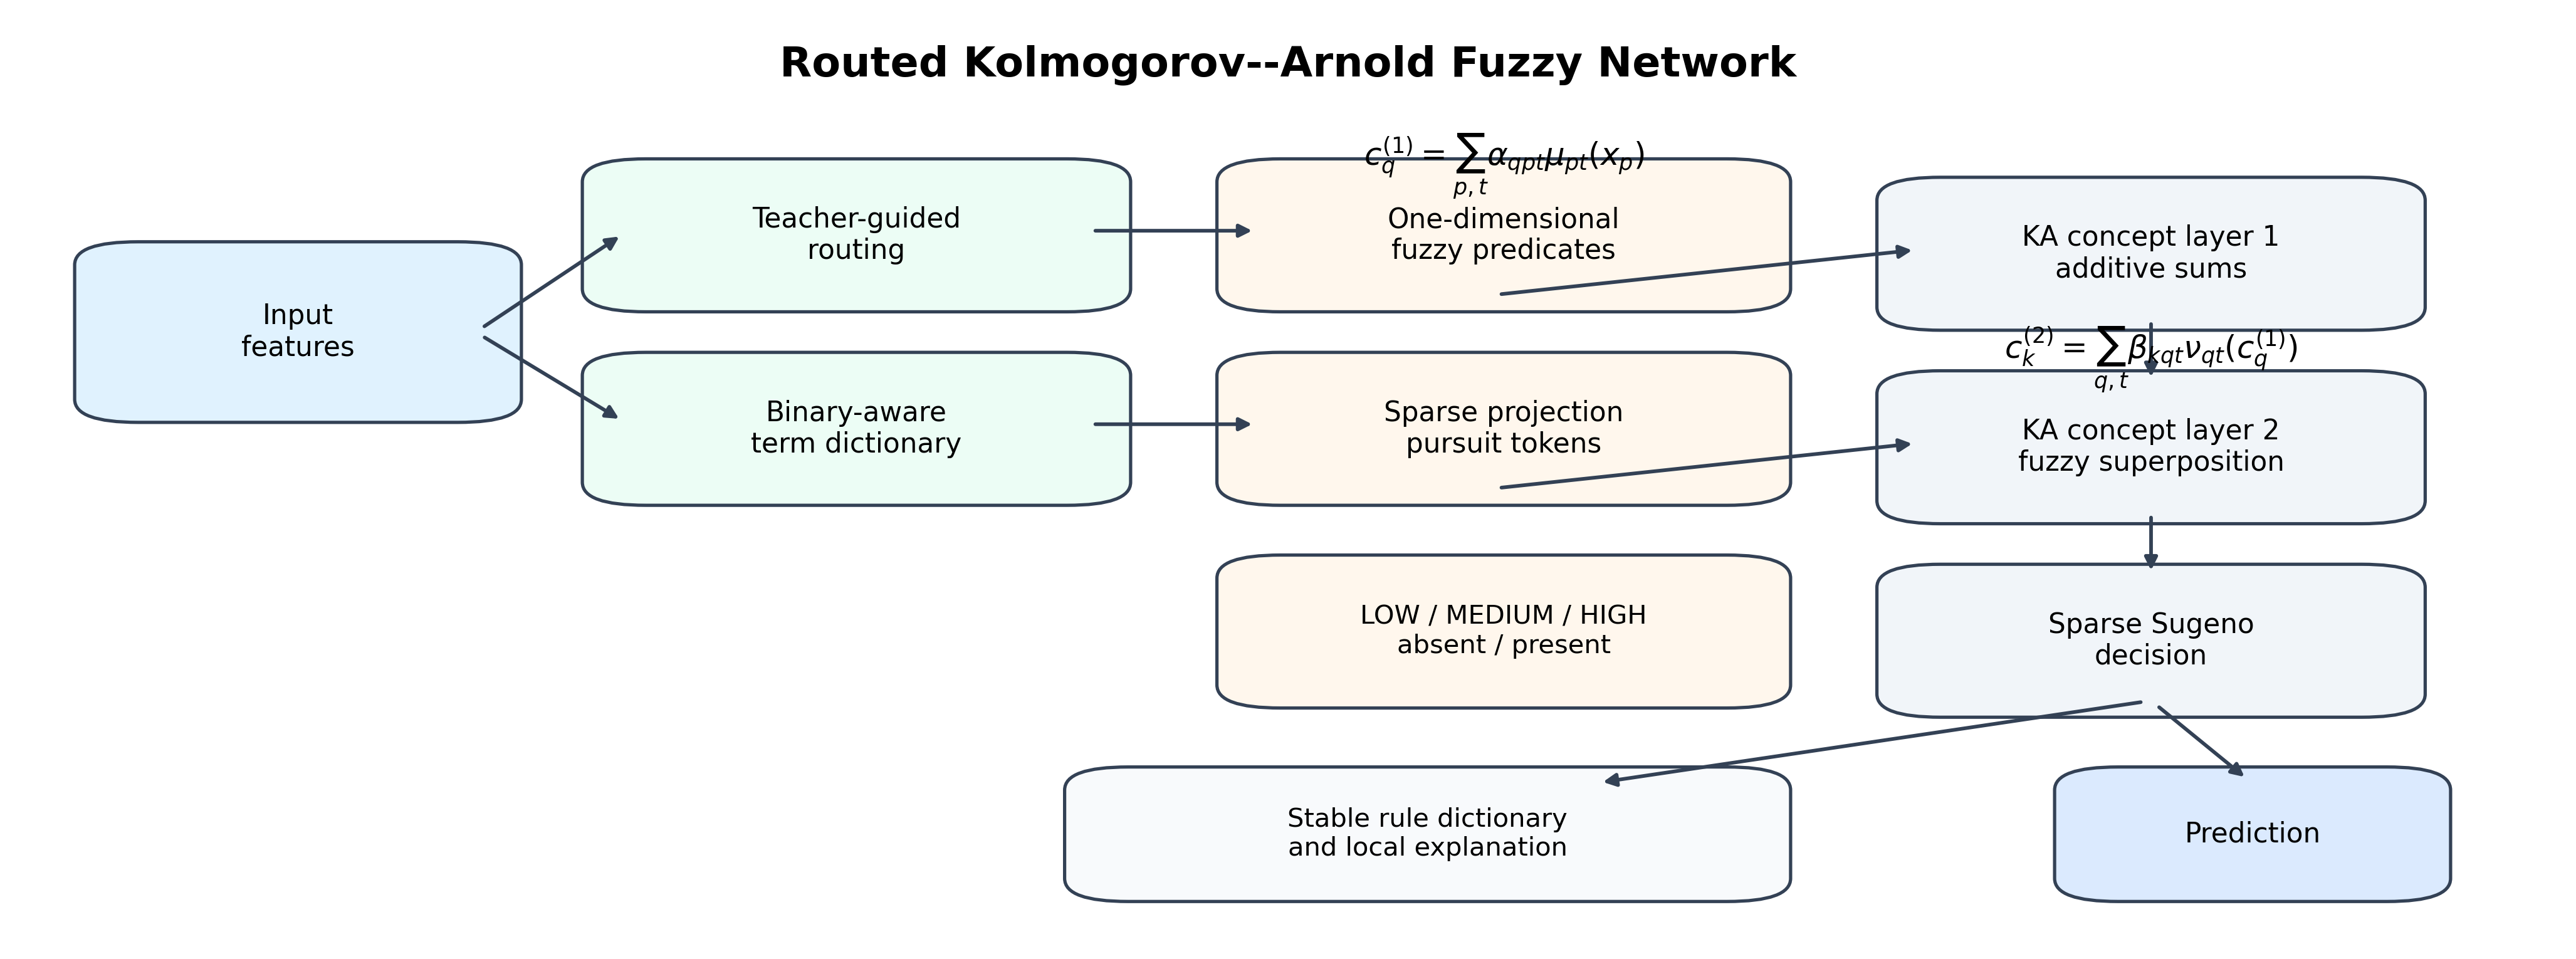
\includegraphics[width=\textwidth]{fig5_kafn_architecture.png}
    \caption{Routed KAFN architecture: teacher-guided routing, binary-aware fuzzy terms, sparse projection-pursuit channels, additive KA concept layers, and sparse Sugeno decision.}
    \label{fig:kafn_architecture}
\end{figure}

Structural complexity is treated as an explicit architectural property rather than as a secondary implementation detail. In a flat global rule base, the number of candidate rules grows rapidly with input dimensionality. Local processing and restricted rule length reduce this growth and make it possible to analyze complexity as a measurable structural cost.

Training is performed within a unified optimization framework, but DFFL is considered in two regimes. In the one-phase regime, all trainable components are optimized jointly after initialization. In the refined regime, training is staged: initialization is followed by concept-level pretraining, rule-base re-estimation in the updated representation space, and final fine-tuning. The purpose of this staged procedure is to stabilize the internal representation and make the hidden rule structure more reproducible across runs.

The overall objective combines task performance with structural regularization,
\[
\mathcal{L} =
\mathcal{L}_{\mathrm{task}}
+ \lambda_{\mathrm{s}}\mathcal{L}_{\mathrm{sparse}}
+ \lambda_{\mathrm{l}}\mathcal{L}_{\mathrm{len}}
+ \lambda_{\mathrm{ord}}\mathcal{L}_{\mathrm{order}}
+ \lambda_{\mathrm{ov}}\mathcal{L}_{\mathrm{overlap}}
+ \lambda_{\mathrm{c}}\mathcal{L}_{\mathrm{cover}} 
\]
\[
+ \lambda_{\mathrm{ort}}\mathcal{L}_{\mathrm{orth}}
+ \lambda_{\mathrm{b}}\mathcal{L}_{\mathrm{bin}}
+ \lambda_{\mathrm{g}}\mathcal{L}_{\mathrm{gate}}.
\]

Here, $\mathcal{L}_{\mathrm{task}}$ corresponds to the predictive objective, while the remaining terms impose structural constraints related to sparsity, rule length, ordering, overlap control, coverage, concept separation, binarization, and gate usage. Under this formulation, interpretability is encouraged directly during learning rather than added as a post hoc explanation.

The refined DFFL training procedure used in this study starts with initialization of local, aggregate, and decision blocks from data-driven prototypes and predefined rule budgets. After that, we run stage-wise pretraining of concept blocks on the training split, then re-estimate rule candidates in the updated concept spaces and rebuild active block structures. Next, we pretrain the decision layer on fixed concept features and then run joint fine-tuning of all trainable parameters with the unified objective and early stopping. For binary tasks, the final classification threshold is tuned on the validation split.
This staged procedure is specific to DFFL in this paper. Shallow, stacked, and hierarchical models are trained without concept-stage re-estimation.

The empirical evaluation was designed to compare the considered architectures within a unified experimental framework. The benchmark includes tabular regression and binary classification tasks, with a main comparison block on smaller standard data sets and an extended comparison block on larger data sets. For large-scale analysis, we use full \textit{covtype\_binary} as the main discriminative benchmark and \textit{kddcup99\_binary\_10percent} as a feasibility/scalability check with repeated-run stability reporting. We also report an additional discriminative large-scale check on \textit{SUSY-200k}.

Reproducibility settings are fixed as follows: three seeds ($19,23,29$), test split $0.2$, validation split $0.2$ (from the original data), feature scaling by MinMax normalization to $[0,1]$, and target scaling to $[0,1]$ for regression tasks. The same seed-specific data split is used for all compared models.

For regression tasks, predictive quality is assessed by the root mean squared error (RMSE). For binary classification, the main metric is the F1 score. Since the study addresses predictive accuracy together with interpretable depth, the evaluation also includes structural and stability-oriented measures. In particular, we record the total number of rules, the number of active rules, and the Jaccard similarity of active-rule configurations across repeated runs.

The comparison includes the four reference neuro-fuzzy architectures and the proposed Routed KAFN. To place their predictive performance in a broader context, we also include standard machine-learning baselines, including linear models, random forests, multilayer perceptrons, Extra Trees, and Histogram Gradient Boosting.

For fuzzy models, the optimization budget is controlled by common defaults: pretraining epochs $18$, decision-pretraining epochs $14$, maximum epochs $80$, patience $20$, and batch size $64$. In binary tasks, the default classification threshold is $0.5$ and can be tuned on validation data in $[0.05,0.95]$. Hyperparameters are selected on validation splits under fixed family-specific search spaces and fixed trial budgets. For fairness, all compared models within each run use the same seed-specific split and fixed per-family budget policies. Standard ML baselines are evaluated on the same splits with fixed model configurations. Resolved settings, including regularization coefficients, are reported in the reproducibility artifacts.

A structured reproducibility package is provided with the manuscript materials and includes resolved run configurations, seeds, metric tables, and figure-generation inputs (\href{https://github.com/lebedeffson/deep-neuro-fuzzy/tree/main/docs/article_current}{article bundle}, \href{https://github.com/lebedeffson/deep-neuro-fuzzy/tree/main/docs/artifacts}{artifacts}).

In this paper, interpretability is operationalized as \textit{structural interpretability}. It is evaluated at two complementary levels. The first is global and concerns the stability of the internal rule structure across repeated runs. The second is local and concerns the decision path for an individual test object. Together, these two perspectives assess reproducibility and traceability of the internal reasoning process. We do not treat this protocol as a full semantic interpretability validation.

At the global level, interpretability is analyzed through the Jaccard similarity of active rules and decision-layer rules across independent runs. For run $s$, a rule is considered active if $p_r^{(s)}\ge \tau_{\mathrm{act}}$, where $p_r^{(s)}$ is the learned rule probability and $\tau_{\mathrm{act}}=0.5$. If $R_a$ and $R_b$ are active-rule sets from two runs, then
\[
J(R_a,R_b)=\frac{|R_a\cap R_b|}{|R_a\cup R_b|}.
\]
These quantities show whether an architecture tends to recover a stable internal structure rather than a substantially different rule configuration at each training instance. We use this metric as a structural stability proxy and not as a full semantic interpretability measure.

At the local level, interpretability is examined through a case-level analysis of a single test object. For Routed KAFN, the trace follows a fixed sequence: input object, binary-aware membership terms, top one-dimensional predicates and projection predicates, concept-level evidence, decision rules, and final output. Figure~\ref{fig:case_explainability_flow} illustrates this logic.

To improve semantic readability beyond index-level tracing, routed predicates are mapped back to original feature names, term labels, and fixed projection-channel definitions in the case-level supplementary artifact.

\begin{figure}[H]
    \centering
    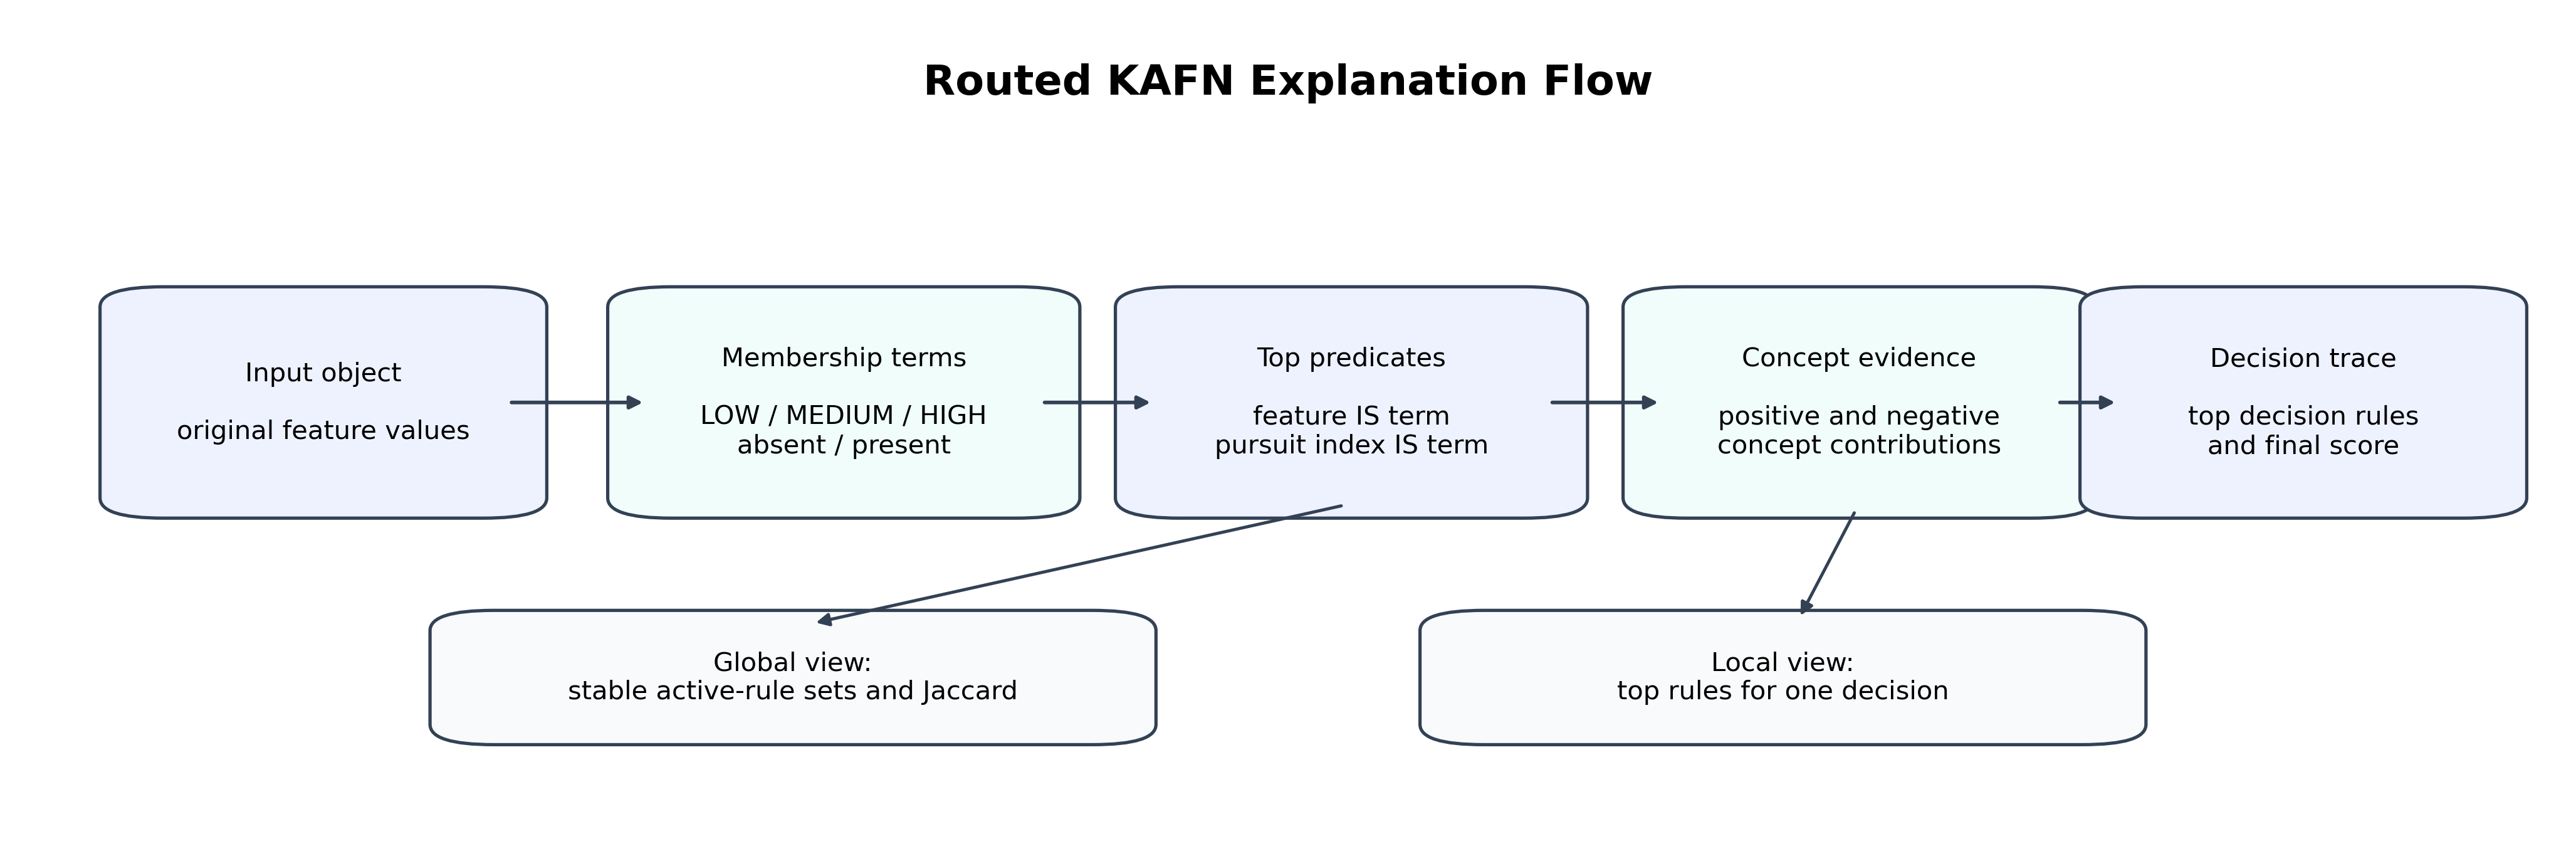
\includegraphics[width=\textwidth]{fig6_kafn_explanation_flow.png}
    \caption{Case-level explainability flow in Routed KAFN: from the input object through membership terms and top predicates to concept evidence, decision rules, and the final score.}
    \label{fig:case_explainability_flow}
\end{figure}

In the present study, the local analysis is demonstrated on the focused \textit{covtype\_binary\_20000} setting, where Routed KAFN is the main proposed model. The first level of the architecture is dominated by routed feature predicates and optional sparse projection predicates, so the input is processed through a fixed, named rule dictionary rather than through a seed-dependent hidden rule topology. At the next level, these local signals are compressed into additive KA concept states. By the time the model reaches the output layer, the final prediction is determined by a small group of dominant Sugeno-style decision terms.

The dominant rules involved in this example are summarized in Table~\ref{tab:case_rules}.

\begin{table}[H]
\centering
\caption{Dominant feature-named rule types in the Routed KAFN case-level trace.}
\label{tab:case_rules}
\small
\setlength{\tabcolsep}{4pt}
\begin{tabular}{lcll}
\toprule
Level & Rule & Weight & Role \\
\midrule
Stage 1 & \makecell[l]{\texttt{Elevation IS HIGH} \\ \texttt{OR WildernessArea\_1 IS present}} & reported per object & routed original-feature evidence \\
Stage 1 & \makecell[l]{\texttt{SoilType\_k IS absent/present}} & reported per object & binary-aware one-hot evidence \\
Projection & \makecell[l]{\texttt{pursuit\_m(Elevation, Slope, ...)} \\ \texttt{IS LOW/MEDIUM/HIGH}} & reported per object & sparse interaction evidence \\
Concept & \makecell[l]{\texttt{KA concept q receives positive} \\ \texttt{and negative predicate contributions}} & reported per object & additive concept state \\
Decision & \makecell[l]{\texttt{concept k IS HIGH/LOW} \\ \texttt{with Sugeno coefficient}} & reported per object & final decision contribution \\
\bottomrule
\end{tabular}
\end{table}

Taken together, the global stability analysis and the local case-level trace define a unified interpretability protocol for the compared models. The former shows whether an architecture tends to recover a reproducible internal rule structure across runs, while the latter shows whether this structure can be read as a coherent decision path for an individual object.

\section{Results}

The compared architectures differ along three evaluation dimensions: predictive quality, rule-base complexity, and internal rule stability. In the reference comparison block, stacked shows the strongest average-rank profile, while DFFL remains competitive on selected tasks and no architecture dominates all tasks at once. The focused Covtype experiments then motivate and evaluate Routed KAFN as the final stability-oriented architecture.
The key quantitative evidence is reported in Tables~\ref{tab:main_results}, \ref{tab:extended_results}, \ref{tab:kanfis_covtype}, \ref{tab:kafn_ablation}, \ref{tab:kafn_best_criteria}, \ref{tab:covtype_capacity_check}, \ref{tab:susy_discriminative}, \ref{tab:best_vs_baseline}, and \ref{tab:all_vs_baseline}.
Values in Tables~\ref{tab:main_results}--\ref{tab:all_vs_baseline} are reported as mean $\pm$ standard deviation across three seeds, except entries explicitly marked as single-seed checks; complete run settings and outputs are provided in the reproducibility artifacts.
For transparency, Table~\ref{tab:main_results} uses one unified reference run for the four baseline neuro-fuzzy architectures. The Routed KAFN row is taken from the dedicated three-seed KAFN run \texttt{runs/kafn\_paper\_all\_3s\_2026-04-30}, which uses the same seeds and split protocol but a KAFN-specific routed configuration.

\begin{table}[H]
\centering
\caption{Summary results of the compared architectures in the main comparison block (mean $\pm$ std over three seeds).}
\label{tab:main_results}
\scriptsize
\setlength{\tabcolsep}{1.5pt}
\begin{tabular}{lllccccc}
\toprule
Model & \makecell[c]{Avg.\\ rules} & \makecell[c]{Mean\\ active-rule\\Jaccard} & Diabetes & Linnerud weight & Breast cancer & Wine binary & Digits binary\\
 &  &  & RMSE & RMSE & F1 & F1 & F1 \\
\midrule
shallow model      & 36.00 & 0.2352 & 0.1852$\pm$0.0024 & 0.3519$\pm$0.2209 & 0.9750$\pm$0.0085 & 0.9577$\pm$0.0340 & 0.9367$\pm$0.0141 \\
stacked model      & 50.00 & 0.1268 & 0.1857$\pm$0.0035 & 0.2887$\pm$0.1396 & 0.9841$\pm$0.0064 & 0.9855$\pm$0.0205 & 0.9953$\pm$0.0066 \\
hierarchical model & 75.00 & 0.1766 & 0.1937$\pm$0.0051 & 0.2430$\pm$0.1691 & 0.9722$\pm$0.0102 & 0.9189$\pm$0.0327 & 0.9953$\pm$0.0066 \\
DFFL               & 75.47 & 0.0888 & 0.1796$\pm$0.0032 & 0.2874$\pm$0.2340 & 0.9652$\pm$0.0207 & 0.9564$\pm$0.0372 & 1.0000$\pm$0.0000 \\
Routed KAFN        & 859.20 & 0.8393 & 0.1953$\pm$0.0058 & 0.2730$\pm$0.1620 & 0.9672$\pm$0.0235 & 0.9322$\pm$0.0369 & 0.9910$\pm$0.0127 \\
\bottomrule
\end{tabular}
\end{table}

The extended comparison shows the same trade-off at larger scale. Stacked remains strongest on \textit{california\_housing}, while Routed KAFN reaches the same mean F1 as hierarchical on \textit{covtype\_binary\_20000} and gives the highest active-rule stability in this two-dataset block.

\begin{table}[H]
\centering
\caption{Summary results of the compared architectures in the extended comparison (mean $\pm$ std over three seeds).}
\label{tab:extended_results}
\small
\setlength{\tabcolsep}{6pt}
\begin{tabular}{lcccc}
\toprule
Model & Avg. rules & \makecell[c]{Mean active-rule\\Jaccard} & California housing & Covtype binary \\
 &  &  & RMSE & F1 \\
\midrule
shallow model      & 36  & 0.3841 & 0.1321$\pm$0.0010 & 0.7101$\pm$0.0183 \\
stacked model      & 50  & 0.1559 & 0.1193$\pm$0.0066 & 0.8129$\pm$0.0108 \\
hierarchical model & 90  & 0.2343 & 0.1233$\pm$0.0044 & 0.8117$\pm$0.0052 \\
DFFL               & 115.67 & 0.2712 & 0.1285$\pm$0.0013 & 0.7518$\pm$0.0046 \\
Routed KAFN        & 888.00 & 0.9463 & 0.1271$\pm$0.0023 & 0.8117$\pm$0.0053 \\
\bottomrule
\end{tabular}
\end{table}

After adding a validation-based rollback safeguard to the hard fine-tuning stage, we additionally re-ran a focused three-seed check on \textit{covtype\_binary\_20000}. The ranking of the reference fuzzy architectures remained unchanged: stacked F1 $=0.8222\pm0.0074$, hierarchical F1 $=0.8037\pm0.0058$, DFFL F1 $=0.7840\pm0.0078$, and shallow F1 $=0.7645\pm0.0030$. Thus, the implementation fix improves reliability of training behavior without changing the main comparative conclusion on this data regime.

The proposed Routed KAFN is evaluated in the same focused Covtype setting because this benchmark exposes the main tension between predictive quality and rule stability. The final configuration uses $Q=12$ first-stage concepts, grouped teacher-guided routing, fan-in $20$, binary-aware fuzzy terms, calibrated threshold tuning, and eight fixed projection-pursuit channels of width four. The non-projection binary-aware variant keeps only 780 active rules and gives the highest structural stability, while the projection variant gives the strongest KAFN predictive result.

\begin{table}[H]
\centering
\caption{Focused \textit{covtype\_binary\_20000} comparison of reference fuzzy models, tree baselines, and Routed KAFN variants.}
\label{tab:kanfis_covtype}
\scriptsize
\setlength{\tabcolsep}{2pt}
\begin{tabular}{lcccccl}
\toprule
Model & F1 & ROC-AUC & PR-AUC & Active rules & Jaccard & Comment \\
\midrule
shallow fuzzy & 0.7645$\pm$0.0030 & 0.8113$\pm$0.0032 & 0.7602$\pm$0.0034 & 18.7 & 0.3493 & compact fuzzy reference \\
DFFL & 0.7840$\pm$0.0078 & 0.8530$\pm$0.0087 & 0.8272$\pm$0.0108 & 73.0 & 0.1077 & concept-oriented reference \\
hierarchical fuzzy & 0.8037$\pm$0.0058 & 0.8809$\pm$0.0055 & 0.8605$\pm$0.0050 & 64.7 & 0.2598 & grouped reference \\
HistGradientBoosting & 0.8154$\pm$0.0065 & 0.8988$\pm$0.0040 & 0.8845$\pm$0.0039 & -- & -- & non-fuzzy baseline \\
Routed KAFN, binary-aware & 0.8165$\pm$0.0067 & 0.8830$\pm$0.0014 & 0.8585$\pm$0.0042 & 780 & 0.9188 & most stable KA variant \\
Routed KAFN, fixed projections & 0.8174$\pm$0.0101 & 0.8857$\pm$0.0035 & 0.8605$\pm$0.0022 & 936 & 0.9167 & final KA variant \\
stacked fuzzy & 0.8222$\pm$0.0074 & 0.8902$\pm$0.0066 & 0.8643$\pm$0.0091 & 20.7 & 0.0978 & strongest fuzzy F1 reference \\
Extra Trees & 0.8546$\pm$0.0026 & 0.9296$\pm$0.0034 & 0.9181$\pm$0.0038 & -- & -- & teacher and upper baseline \\
\bottomrule
\end{tabular}
\end{table}

For the pre-projection teacher-guided grouped KA model, the additional three-seed verification gives ROC-AUC $=0.8848$ and PR-AUC $=0.8595$ at F1 $=0.8166\pm0.0029$ with 936 rules and active-rule Jaccard $=0.9079$. This confirms that the routed additive construction is not only an F1-specific improvement. The binary-aware variant then reduces the active rule base from 936 to 780 and increases Jaccard to $0.9188$ with essentially unchanged F1. The fixed-projection variant is selected as the final KAFN because it gives the best mean F1 among the stable KA configurations while keeping Jaccard above $0.91$.

\begin{table}[H]
\centering
\caption{Ablation path leading to the final Routed KAFN on \textit{covtype\_binary\_20000}.}
\label{tab:kafn_ablation}
\scriptsize
\setlength{\tabcolsep}{3pt}
\begin{tabular}{lcccccl}
\toprule
Variant & F1 & ROC-AUC & PR-AUC & Active rules & Jaccard & Interpretation \\
\midrule
Teacher-guided grouped KA & 0.8166$\pm$0.0029 & 0.8848$\pm$0.0019 & 0.8595$\pm$0.0037 & 936 & 0.9079 & stable base model \\
KA + calibrated threshold & 0.8169$\pm$0.0031 & 0.8848$\pm$0.0019 & 0.8595$\pm$0.0037 & 936 & 0.9079 & threshold-only gain \\
KA + binary-aware terms & 0.8165$\pm$0.0067 & 0.8830$\pm$0.0014 & 0.8585$\pm$0.0042 & 780 & 0.9188 & clearer one-hot logic \\
Routed KAFN + fixed projections & 0.8174$\pm$0.0101 & 0.8857$\pm$0.0035 & 0.8605$\pm$0.0022 & 936 & 0.9167 & final trade-off \\
\bottomrule
\end{tabular}
\end{table}

The final KA variant does not overtake the stacked fuzzy model in mean F1, but it changes the quality--interpretability balance. Compared with stacked fuzzy, it loses about $0.0048$ F1 while increasing active-rule Jaccard from $0.0978$ to $0.9167$. Compared with histogram gradient boosting, it gives a slightly higher mean F1 in this focused block and provides explicit fuzzy rules. Compared with the binary-aware KA variant, the projection extension adds interaction capacity and improves mean F1 from $0.8165$ to $0.8174$, at the cost of increasing active rules from 780 to 936.

\begin{table}[H]
\centering
\caption{Best observed values by criterion in the focused \textit{covtype\_binary\_20000} block.}
\label{tab:kafn_best_criteria}
\scriptsize
\setlength{\tabcolsep}{4pt}
\begin{tabular}{lll}
\toprule
Criterion & Best model & Value \\
\midrule
Best overall F1 & Extra Trees & 0.8546$\pm$0.0026 \\
Best fuzzy F1 & stacked fuzzy & 0.8222$\pm$0.0074 \\
Best stable fuzzy F1, $J>0.9$ & Routed KAFN, fixed projections & 0.8174$\pm$0.0101 \\
Best active-rule Jaccard & Routed KAFN, binary-aware & 0.9188 \\
Best final-model Jaccard & Routed KAFN, fixed projections & 0.9167 \\
Best non-fuzzy baseline below Extra Trees & HistGradientBoosting & 0.8154$\pm$0.0065 \\
\bottomrule
\end{tabular}
\end{table}

Thus, the metric where the proposed family is best is structural stability: both KAFN variants exceed $0.91$ active-rule Jaccard. The final fixed-projection KAFN is also the best stable fuzzy classifier in this block and slightly exceeds histogram gradient boosting in mean F1, but it is not the absolute F1 leader.

When the analysis shifts from predictive quality to internal rule stability, the picture changes. In the current quality-oriented DFFL setting, active-rule Jaccard in the main block is lower than in the strongest stability-oriented variants, which indicates that quality-focused tuning can reduce reproducibility of internal active-rule configurations.

Because the larger Covtype task suggested that the reference stacked model may be capacity-limited, we additionally ran a targeted large-scale capacity check on the full \textit{covtype\_binary} data set with 581,012 samples. This check is reported separately from the unified reference comparison because it uses an enhanced stacked configuration: larger hidden width and rule budget (factor $3.0$), a gated final skip from 32 selected raw features, distillation from an Extra Trees teacher (blend weight $0.15$), and a second-stage error-focused fine-tuning. The result is a stronger stacked variant with 150 rules and 33 hidden concepts.

\begin{table}[H]
\centering
\caption{Large-scale results on full \textit{covtype\_binary} (three-seed results).}
\label{tab:covtype_capacity_check}
\scriptsize
\setlength{\tabcolsep}{4pt}
\begin{tabular}{lccccc}
\toprule
Model & F1 & ROC-AUC & PR-AUC & Rules & Active-rule Jaccard \\
\midrule
stacked (enhanced)& 0.9466$\pm$0.0015 & 0.9895$\pm$0.0005 & 0.9886$\pm$0.0005 & 150 & 0.1625 \\
DFFL & 0.8478$\pm$0.0037 & 0.9246$\pm$0.0033 & 0.9149$\pm$0.0037 & 144 & 0.0222 \\
hierarchical (enhanced)& 0.8930$\pm$0.0004 & 0.9615$\pm$0.0009 & 0.9573$\pm$0.0013 & 207 & 0.2050 \\
hist gradient boosting & 0.8328$\pm$0.0011 & 0.9183$\pm$0.0010 & 0.9099$\pm$0.0012 & -- & -- \\
MLP & 0.8589$\pm$0.0009 & 0.9377$\pm$0.0026 & 0.9307$\pm$0.0029 & -- & -- \\
extra trees & 0.9543$\pm$0.0003 & 0.9919$\pm$0.0001 & 0.9912$\pm$0.0002 & -- & -- \\
random forest & 0.9560$\pm$0.0001 & 0.9924$\pm$0.0001 & 0.9918$\pm$0.0001 & -- & -- \\
\bottomrule
\end{tabular}
\end{table}

The capacity-tuned stacked model substantially improves over the smaller reference configurations and becomes stronger than histogram gradient boosting, MLP, and the tested hierarchical fuzzy variant on full Covtype. However, it remains below Random Forest and Extra Trees. DFFL in the current three-seed run reaches F1 $=0.8478\pm0.0037$, which is above histogram gradient boosting but below MLP, stacked, and tree ensembles.

Routed KAFN is not included in Table~\ref{tab:covtype_capacity_check}, because a completed full-\textit{covtype\_binary} KAFN run was not available for the same full-scale block. Its validated large-tabular result in this manuscript is the focused \textit{covtype\_binary\_20000} block reported in Tables~\ref{tab:kanfis_covtype}--\ref{tab:kafn_best_criteria}.

As an additional fairness-oriented diagnostic, we ran a capacity-matched fuzzy-only setting on full Covtype under a unified fast budget. In this setting, stacked and DFFL use near-matched total rules (106 and 107 respectively), while hierarchical uses 171 rules in the same budget regime. Stacked remains the strongest fuzzy variant (F1 $=0.9049\pm0.0043$), followed by hierarchical (F1 $=0.8540\pm0.0051$) and DFFL (F1 $=0.8021\pm0.0075$). This diagnostic indicates that, in the current implementation, DFFL does not close the quality gap to stacked even when the rule-budget comparison is constrained.

As a secondary large-scale sanity check, we evaluate \textit{kddcup99\_binary\_10percent}. In this check, fuzzy models reach near-saturated F1 values: shallow $0.9965\pm0.0006$, stacked $0.9995\pm0.0001$, hierarchical $0.9995\pm0.0001$, and DFFL $0.9993\pm0.0001$. This setting confirms feasibility and repeated-run behavior, but it is weakly discriminative because most methods approach perfect scores. For this reason, we do not use KDD as a primary quality separator in the main comparative interpretation.

To reduce the near-perfect saturation effect observed on KDD, we add a more discriminative large-scale check on \textit{SUSY-200k}. Fuzzy-model values are reported over three seeds, while baseline values are a single-seed snapshot (seed 23) and are therefore treated as contextual rather than significance-tested comparisons.

\begin{table}[H]
\centering
\caption{Additional discriminative large-scale check on \textit{SUSY-200k}.}
\label{tab:susy_discriminative}
\scriptsize
\setlength{\tabcolsep}{4pt}
\begin{tabular}{lcccc}
\toprule
Model & F1 & ROC-AUC & PR-AUC & Seeds \\
\midrule
shallow fuzzy & 0.7626$\pm$0.0062 & 0.8582$\pm$0.0072 & 0.8602$\pm$0.0092 & 3 \\
stacked fuzzy & 0.7713$\pm$0.0039 & 0.8685$\pm$0.0039 & 0.8725$\pm$0.0042 & 3 \\
hierarchical fuzzy & 0.7708$\pm$0.0047 & 0.8688$\pm$0.0032 & 0.8738$\pm$0.0028 & 3 \\
DFFL & 0.7718$\pm$0.0020 & 0.8688$\pm$0.0021 & 0.8728$\pm$0.0015 & 3 \\
logistic regression & 0.7395 & 0.8556 & 0.8595 & 1 \\
hist gradient boosting & 0.7655 & 0.8745 & 0.8789 & 1 \\
mlp classifier & 0.7687 & 0.8736 & 0.8787 & 1 \\
\bottomrule
\end{tabular}
\end{table}

Routed KAFN is likewise not reported in the SUSY table, because the available completed SUSY run predates the final KAFN configuration. We therefore do not transfer the focused Covtype KAFN numbers to SUSY.

To evaluate robustness, we report nonparametric tests on benchmark summaries: a Friedman test with pairwise Wilcoxon signed-rank tests and Holm correction. In the main block, the dataset-level Friedman test is not significant ($\chi^2=2.04$, $p=0.6327$). In the extended block, it is significant ($\chi^2=6.00$, $p=0.0383$), but no pairwise comparison remains significant after Holm correction at $\alpha=0.05$.
These tests are computed on the unified three-seed benchmark blocks, while the separate full-Covtype capacity table is treated as a diagnostic and excluded from significance testing.

Because active-rule stability depends on the activation threshold $\tau_{\mathrm{act}}$, we additionally ran a threshold-sensitivity check on the main benchmark block with $\tau\in\{0.3,0.5,0.7\}$. At $\tau=0.3$, mean active-rule Jaccard across datasets is 0.4511 (stacked), 0.4381 (hierarchical), and 0.2261 (DFFL). At the default $\tau=0.5$, the same values are 0.1218, 0.1640, and 0.2198. At $\tau=0.7$, stacked and hierarchical saturate at 1.0 in this fast setting due to the very sparse surviving active-rule sets, while DFFL remains at 0.2090. This supplementary fast-setting check is threshold-sensitive and does not replace the main reference comparison in Table~\ref{tab:main_results}. We therefore keep $\tau_{\mathrm{act}}=0.5$ as the default reporting point and interpret high-$\tau$ values with caution.

The comparison with external baselines is included to contextualize raw predictive performance. The main contribution of this study is the Routed KAFN architecture and its evaluation against both neuro-fuzzy and non-fuzzy baselines under a multi-criteria protocol. The earlier shallow, stacked, hierarchical, and DFFL models remain important because they show why a routed additive KA structure is useful: stacked models are accurate but structurally unstable, while concept-oriented DFFL is traceable but does not close the Covtype quality gap.

\begin{table}[H]
\centering
\caption{Neuro-fuzzy results in the context of standard ML baselines (mean $\pm$ std over three seeds).}
\label{tab:best_vs_baseline}
\scriptsize
\setlength{\tabcolsep}{2pt}
\begin{tabular}{lclclcl}
\toprule
Dataset & Metric & Best neuro-fuzzy model & Value & Routed KAFN & Best baseline & Value \\
\midrule
diabetes               & RMSE & DFFL               & 0.1796$\pm$0.0032 & 0.1953$\pm$0.0058 & linear regression        & 0.1779$\pm$0.0025 \\
linnerud\_weight       & RMSE & hierarchical model & 0.2430$\pm$0.1691 & 0.2730$\pm$0.1620 & hist gradient boosting   & 0.3058$\pm$0.1508 \\
breast\_cancer         & F1   & stacked model      & 0.9841$\pm$0.0064 & 0.9672$\pm$0.0235 & extra trees classifier   & 0.9908$\pm$0.0032 \\
wine\_binary           & F1   & stacked model      & 0.9855$\pm$0.0205 & 0.9322$\pm$0.0369 & extra trees classifier   & 1.0000$\pm$0.0000 \\
digits\_binary         & F1   & DFFL               & 1.0000$\pm$0.0000 & 0.9910$\pm$0.0127 & mlp classifier           & 1.0000$\pm$0.0000 \\
california\_housing    & RMSE & stacked model      & 0.1193$\pm$0.0066 & 0.1271$\pm$0.0023 & hist gradient boosting   & 0.0972$\pm$0.0014 \\
covtype\_binary\_20000 & F1   & stacked fuzzy      & 0.8222$\pm$0.0074 & 0.8174$\pm$0.0101 & extra trees classifier   & 0.8546$\pm$0.0026 \\
\bottomrule
\end{tabular}
\end{table}

\begin{table}[H]
\centering
\caption{Reference neuro-fuzzy architectures and Routed KAFN against the best external baseline per data set (signed delta; positive is better). For RMSE, positive means lower error than the baseline; for F1, positive means higher F1. The Covtype row uses the focused three-seed block.}
\label{tab:all_vs_baseline}
\scriptsize
\setlength{\tabcolsep}{3pt}
\begin{tabular}{lclccccc}
\toprule
Dataset & Metric & Best baseline & Shallow & Stacked & Hierarchical & DFFL & Routed KAFN \\
\midrule
diabetes               & RMSE & linear regression                 & -0.0073 & -0.0079 & -0.0158 & -0.0017 & -0.0174 \\
linnerud\_weight       & RMSE & hist gradient boosting & -0.0462 & +0.0170 & +0.0628 & +0.0183 & +0.0328 \\
breast\_cancer         & F1   & extra trees classifier           & -0.0159 & -0.0067 & -0.0186 & -0.0256 & -0.0236 \\
wine\_binary           & F1   & extra trees classifier           & -0.0423 & -0.0145 & -0.0811 & -0.0436 & -0.0678 \\
digits\_binary         & F1   & mlp classifier                   & -0.0633 & -0.0047 & -0.0047 & +0.0000 & -0.0090 \\
california\_housing    & RMSE & hist gradient boosting & -0.0349 & -0.0221 & -0.0262 & -0.0313 & -0.0299 \\
covtype\_binary\_20000 & F1   & extra trees classifier           & -0.0901 & -0.0324 & -0.0509 & -0.0706 & -0.0372 \\
\bottomrule
\end{tabular}
\end{table}

As shown in Table~\ref{tab:all_vs_baseline}, the reference neuro-fuzzy models outperform the best external baseline on \textit{linnerud\_weight}. Routed KAFN is also better than the external baseline on \textit{linnerud\_weight}, but on the remaining tasks it is below the strongest external baseline. In the focused Covtype block it is close to stacked fuzzy and above histogram gradient boosting, but it remains below Extra Trees.

Overall, the results point to a trade-off rather than a single best architecture. Stacked leads the main reference block by average rank and still has the highest focused Covtype F1 among fuzzy models. Routed KAFN, however, gives the strongest stability-oriented result in the focused Covtype block, combining near-stacked F1 with active-rule Jaccard above $0.91$.

The KAFN ablation leads to the same general conclusion. Adding binary-aware terms and fixed projection channels changes the quality--stability balance without making KAFN an absolute F1 leader; the strongest contribution is the stable routed rule topology.

\section{Discussion}

The comparison shows a stable pattern. Different forms of depth in neuro-fuzzy systems support different objectives, and no single architecture dominates all criteria at once. Sequential and hierarchical organizations remain strong in predictive terms, while DFFL clarifies the limits of concept-oriented decomposition. Routed KAFN is introduced as the final response to this limitation: it keeps a deep concept structure, but avoids high-order fuzzy products by using routed additive one-dimensional predicates.

The full Covtype capacity check clarifies this point at implementation level. The reference stacked setup was constrained by optimization settings and by the available rule and concept capacity. After increasing capacity and adding a gated raw-feature skip, stacked reached the strongest fuzzy result on this large task. At the same time, the gain required a larger rule budget and came with lower active-rule Jaccard, so the quality gain was achieved through a clear trade-off between quality, complexity, and stability.

Within the same Covtype setting, DFFL remains below the capacity-tuned stacked variant. This suggests that the original DFFL configuration still needs stronger bridge and aggregation capacity to preserve cross-feature information more effectively in high-dimensional tabular data. Routed KAFN addresses this issue more directly: teacher-guided routes preserve feature-level access, binary-aware terms remove uninformative predicates for one-hot variables, and fixed projection channels add a small controlled interaction layer.

Runtime measurements support the same interpretation. Under matched fast settings on full Covtype (seed 23), stacked was fastest in training at 69.57s, hierarchical was intermediate at 122.58s, and DFFL was slowest at 423.89s. Inference with evaluation remained in the same low-second range for all three methods, around 2--3s. In this regime, the current DFFL implementation requires substantially more training time than stacked, while its predictive advantage is not realized on full Covtype.

This is important for the main claim of the paper. If interpretability is treated as a property of internal reasoning rather than an external post hoc explanation, then evaluation cannot be reduced to RMSE or F1. Reproducibility of internal rule structure becomes a necessary criterion alongside predictive quality. This is where Routed KAFN gives its clearest advantage: the final projection variant reaches active-rule Jaccard $0.9167$, while the stronger-F1 stacked fuzzy model reaches only $0.0978$ in the focused Covtype check.

The current DFFL results should therefore be interpreted as an architectural operating regime rather than as a uniform accuracy gain. In these experiments, quality-oriented tuning gives the best fuzzy value on \textit{diabetes} (RMSE) and \textit{digits\_binary} (F1), while the model remains below the strongest external baselines on several tasks and shows lower active-rule reproducibility in the main block. Routed KAFN changes this conclusion for the focused Covtype analysis: it does not beat Extra Trees and does not fully overtake stacked fuzzy, but it reaches the histogram-gradient-boosting level while preserving a stable named rule structure.

One likely mechanism behind this trade-off is the early local decomposition used in DFFL. It reduces combinatorial rule growth, but it also creates an early information bottleneck because upper layers operate on aggregated local representations rather than the full original feature space. Routed KAFN reduces this bottleneck by routing teacher-ranked original predicates into each concept and by adding fixed projection-pursuit channels for limited cross-feature evidence.

The baseline comparison reinforces the practical reading of the results. Standard machine-learning models often remain stronger in raw predictive metrics, especially Extra Trees on Covtype. The value of Routed KAFN lies in a different operating point: explicit fuzzy predicates, reproducible routed topology, readable binary terms, and a stable set of active rules with competitive F1.

\section{Limitations}

The main limitation is empirical scope. The current evidence is restricted to tabular tasks; extension to image, text, and other modalities requires dedicated validation under modality-specific pipelines.

The second limitation concerns semantic validation depth. In this paper, interpretability is evaluated primarily in structural terms through rule sets, rule counts, stability, and case-level traceability. This provides reproducible internal diagnostics, but full domain-expert assessment of concept meaning remains an important next stage.

The third limitation concerns large-scale efficiency. The large-scale results are mixed. DFFL remains competitive with the strongest fuzzy variants on SUSY-200k, and the KDD feasibility check confirms that the model can be trained and evaluated in a larger setting. At the same time, full Covtype exposes a harder regime for the present configuration. Routed KAFN is currently validated as a focused Covtype-20k improvement; full-scale KAFN evaluation remains future work.

\section{Conclusion}

This paper examined how to increase complexity in neuro-fuzzy models while preserving structural interpretability of internal reasoning. We developed, formalized, and implemented a set of fuzzy-network architectures in one framework and used them to motivate the final Routed KAFN design. The results show that different forms of depth lead to systematically different balances between predictive quality, structural complexity, and internal rule stability.

The study presents Routed KAFN as a teacher-guided Kolmogorov--Arnold fuzzy network with binary-aware fuzzy terms and fixed projection-pursuit channels. On \textit{covtype\_binary\_20000}, the final KAFN variant reaches F1 $=0.8174\pm0.0101$ with active-rule Jaccard $=0.9167$. This is close to stacked fuzzy in F1 and much stronger in rule-structure reproducibility.

These findings imply that architecture selection in deep neuro-fuzzy modeling should be treated as a joint optimization problem, where predictive accuracy, rule-base size, reproducibility of internal rule structure, and runtime efficiency are considered together.

Further work should scale Routed KAFN to the full Covtype setting, strengthen projection-route selection, and add domain-expert validation of the named concepts and local rule traces beyond structural stability metrics.

\bibliographystyle{splncs04}
\bibliography{docs/iiti26_references_skeleton_en}

\end{document}
